\section{对偶理论}
\subsection{LP对偶问题的形式}
\subsection{LP的对偶定理}
\subsection{对偶问题的经济解释}
\subsection{对偶单纯形法}
\subsection{原-对偶算法}
原-对偶算法不考。

\begin{note}
    对称形式的对偶规划的要点
    \begin{itemize}
        \item min变成max,价值系数 $c$ 与右端向量 $b$ 互换,系数矩阵 $A$ 转置,$\ge$ 变为 $\le$
        \item 原问题中约束条件的个数 = 对偶问题中变量的个数
        \item 原问题中变量的个数 = 对偶问题中约束条件的个数
        \item $\begin{cases}
            \min \quad &c^Tx\\
            s.t. \quad &Ax \ge b\\
            & x \ge 0
        \end{cases}\quad  \Longrightarrow \quad \begin{cases}
            \max\quad &b^Tw \\
            s.t.\quad &A^Tw \le c\\
            &w \ge 0
        \end{cases}$
        \item 对偶问题的对偶问题是原问题
        \item 一般情形 LP 问题的对偶问题\[\begin{cases}
            \min \quad & c^Tx\\
            s.t. \quad & A_1x \ge b_1\\
            & A_2x = b_2\\
            &A_3x \le b_3\\
            &x \ge 0
        \end{cases} \quad \Longrightarrow \quad \begin{cases}
            \max \quad & b_1^Tw_1 + b_2^Tw_2 + b_3^Tw_3\\
            s.t. \quad & A_1^Tw_1 + A_2^Tw_2 + A_3^Tw_3 \le c\\
            &w_1 \ge 0, w_2\  \text{free}, w_3 \le 0
        \end{cases}\]
        图\ref{fig2}中,右边是原问题,左边是对偶问题.
        \begin{figure}[htbp]
            \centering
            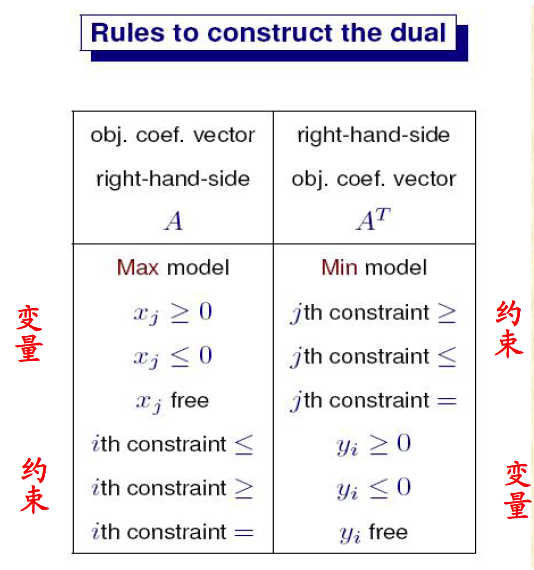
\includegraphics[width=0.4\textwidth]{./figures/img2.png}
            \caption{LP问题的对偶问题转换规则 \label{fig2}}
        \end{figure}
        \[\begin{cases}
            \min \quad & 2x_1 + x_2 + 2x_3\\
            s.t. \quad & x_1 + x_2 + 2x_3 \ge 1\\
            &x_1 - x_2 + x_3 \le 2\\
            &-x_1 + x_2 + x_3 = 1\\
            &x_1 \ge 0, x_2 \ \text{free}, x_3 \le 0
        \end{cases} \Longrightarrow \begin{cases}
            \max \quad & w_1 + 2w_2 + w_3\\
            s.t. \quad & w_1 + w_2 - w_3 \le 2\\
            &w_1 - w_2 + w_3 = 1\\
            &2w_1 + w_2 + w_3 \ge 2\\
            &w_1 \ge 0, w_2 \le 0, w_3 \ \text{free}
        \end{cases}\]
        原问题的变量对应对偶问题的约束,并且\textbf{符号改变}.
    \end{itemize}
\end{note}

\begin{note}
    对偶问题的基本性质
    \begin{itemize}
        \item 弱对偶定理:若 $x^{(0)}, w^{(0)}$ 分别是原问题(P)和对偶问题(D)的可行解,则 $c^Tx^{(0)} \ge b^Tw^{(0)}$,即最小化目标的函数值大于等于最大化目标的函数值.\begin{itemize}
            \item Proof:\begin{itemize}
                \item $Ax^{(0)} \ge b, x^{(0)} \ge 0$,同时 $A^Tw^{(0)} \le c, w^{(0)} \ge 0$,故 $c^Tx^{(0)} \ge (A^Tw^{(0)})^Tx^{(0)} = (w^{(0)})^TAx^{(0)} \ge (w^{(0)})^Tb = b^Tw^{(0)}$
            \end{itemize}
            \item 推论1:若原问题(P)或对偶问题(D)有无界解,则其对偶问题(D)或原问题(P)无可行解
            \item 推论2:极大化问题的任何一个可行解所对应的目标函数值都是其对偶问题的目标函数值的下界.
            \item 推论3:极小化问题的任何一个可行解所对应的目标函数值都是其对偶问题的目标函数值的上界.
        \end{itemize}
        \item 最优性准则:若 $x^{(0)}, w^{(0)}$ 分别为原问题(P)对偶问题(D)的可行解,且 $cx^{(0)} = w^{(0)}b$,则 $x^{(0)}, w^{(0)}$ 分别为原问题(P)对偶问题(D)的最优解
        \item 强对偶定理:若原问题(P)和对偶问题(D)均有可行解,则原问题(P)和对偶问题(D)均有最优解,且(P)(D)的最优目标函数值相等.\begin{itemize}
            \item 推论:若问题(P)或(D)无可行解,则其对偶问题(D)或(P)或者无可行解,或者目标函数值趋于无穷.
            \item 推论:在用单纯形法求解LP问题(P)的最优单纯形表中松弛变量的检验数的相反数为单纯形乘子$w = c_BB^{-1}$,也就是其对偶问题(D)的最优解.
        \end{itemize}
    \end{itemize}
\end{note}

\begin{note}
    总结:
    \begin{itemize}
        \item 原问题有最优解,对偶问题一定有最优解,且相同
        \item 原问题有无界解,则对偶问题无可行解
        \item 原问题无可行解,则对偶问题有无界解或无可行解
    \end{itemize}
\end{note}

\begin{note}
    互补松弛定理:设 $x^{(0)}, w^{(0)}$ 分别是 (P), (D) 问题的可行解,则 $x^{(0)},w^{(0)}$ 分别为 (P), (D) 的最优解的充要条件是 $\forall i, j (1 \le i \le m, 1\le j \le n)$ 有 \begin{itemize}
        \item 若 $x_j^{(0)} > 0$,则 $w^{(0)}P_j = c_j$
        \item 若 $w^{(0)}P_j < c_j$,则 $x_j^{(0)} = 0$
        \item 若 $w_i^{(0)} > 0$,则 $A_ix^{(0)} = b_i$
        \item 若 $A_ix^{(0)} > b_i$,则 $w_i^{(0)} = 0$
    \end{itemize}
    即 $\begin{cases}
        (c - w^{(0)}A)x^{(0)} = 0\\
        w^{(0)}(Ax^{(0)} - b) = 0
    \end{cases}$,其中 $P_j$ 是 $A$ 的第 $j$ 列,$A_i$ 是 $A$ 的第 $i$ 行.

    互补松弛定理(非对称形式)

    设 $x^{(0)}$ 和 $w^{(0)}$ 分别是 $\begin{cases}
        \min \quad & c^Tx \\
        s.t. \quad & Ax = b\\
        &x \ge 0
    \end{cases}$ 和 $\begin{cases}
        \max \quad & b^Tw \\
        s.t. \quad & A^Tw \le c
    \end{cases}$ 的可行解,则 $x^{(0)}$ 和 $w^{(0)}$ 是最优解的充要条件是 $\forall j$ \begin{itemize}
        \item $x_j^{(0)} > 0 \Longrightarrow w^{(0)}P_j = c_j$
        \item $w^{(0)}P_j < c_j \Longrightarrow x_j^{(0)} = 0$
    \end{itemize}
\end{note}

\begin{note}
    对偶单纯形法步骤:
    \begin{enumerate}
        \item 化标准型,建立初始单纯形表
        \item 判断,若 $B^{-1}b \ge 0$,则已得到最优解
        \item 换基迭代 \begin{enumerate}
            \item 确定换出变量,$\bar{b_r} = \min_i\left\{\bar{b_i}\right\} < 0, x_r$ 为换出变量
            \item 确定换入变量,$\min_{j}\left\{\frac{z_j - c_j}{y_{rj}}\ |\ y_{rj} < 0\right\} = \frac{z_k - c_k}{y_{rk}}$,$x_k$ 为换入变量(若所有 $y_{rj} \ge 0$,则该 LP 问题无可行解)
            \item 换基迭代,$y_{rk}$ 为主元
        \end{enumerate}
        \item 回到第 2 步
    \end{enumerate}
\end{note}

\begin{note}
    对偶单纯形法与原单纯形法的区别:
    \begin{itemize}
        \item 原单纯形法保持原问题的可行性,对偶单纯形法保持所有检验数 $wP_j - c_j \le 0$,即保持对偶问题的可行性.
        \item 特点:先选择出基变量,再选择进基变量.
    \end{itemize}
\end{note}
